%% pyti_lpc_cmd_paper_lua.tex
%% LuaLaTeX version — OpenType fonts via fontspec + unicode-math
%% Academic paper: Architecture and Implementation of pyti_lpc_cmd
%% Copyright (C) 2026 Kris Kirby, KE4AHR  --  Licensed GPLv3.0
%%
\documentclass[10pt]{article}

% ── Packages ────────────────────────────────────────────────────────────────
% LuaLaTeX: inputenc / fontenc / lmodern replaced by fontspec + unicode-math
\usepackage{fontspec}
\setmainfont{Latin Modern Roman}[Ligatures=TeX]
\setsansfont{Latin Modern Sans}[Ligatures=TeX]
\setmonofont{Latin Modern Mono}[Ligatures=TeX, Scale=MatchLowercase]
\usepackage{amsmath}          % load before unicode-math
\usepackage{unicode-math}
\setmathfont{latinmodern-math.otf}
\usepackage[margin=1in]{geometry}
\usepackage{graphicx}
\usepackage{tikz}
\usetikzlibrary{arrows.meta,shapes.geometric,shapes.misc,fit,
                positioning,calc,decorations.pathreplacing,matrix}
\usepackage{pgfplots}
\pgfplotsset{compat=1.18}
\usepackage{listings}
\usepackage{xcolor}
\usepackage{booktabs}
\usepackage{microtype}
\usepackage{hyperref}
\usepackage{caption}
\usepackage{subcaption}
\usepackage{float}
\usepackage{placeins}
\usepackage{needspace}
\usepackage{enumitem}
\usepackage{fancyhdr}
\usepackage{abstract}
\usepackage{titlesec}
\usepackage{appendix}
\usepackage{array}
\usepackage[style=numeric,backend=biber,sorting=none]{biblatex}
\addbibresource{refs.bib}

% ── Colours ─────────────────────────────────────────────────────────────────
\definecolor{codegreen}{rgb}{0.0,0.50,0.0}
\definecolor{codegray}{rgb}{0.45,0.45,0.45}
\definecolor{codeblue}{rgb}{0.0,0.0,0.65}
\definecolor{codeback}{rgb}{0.97,0.97,0.97}
\definecolor{blockblue}{RGB}{220,235,255}
\definecolor{blockgreen}{RGB}{215,245,215}
\definecolor{blockorange}{RGB}{255,235,210}
\definecolor{blockred}{RGB}{255,215,215}
\definecolor{blockgray}{RGB}{235,235,235}
\definecolor{arrowgray}{RGB}{100,100,100}

% ── Listing style ────────────────────────────────────────────────────────────
\lstdefinestyle{pycode}{
  language=Python,
  backgroundcolor=\color{codeback},
  basicstyle=\ttfamily\footnotesize,
  keywordstyle=\color{codeblue}\bfseries,
  commentstyle=\color{codegreen}\itshape,
  stringstyle=\color{codeblue!70!black},
  numberstyle=\tiny\color{codegray},
  numbers=left,
  stepnumber=1,
  numbersep=6pt,
  frame=single,
  framerule=0.4pt,
  breaklines=true,
  breakatwhitespace=true,
  tabsize=4,
  captionpos=b,
  showstringspaces=false,
}
% float=H keeps each listing together on one page (uses float package's H specifier)
\lstset{style=pycode, float=H, floatplacement=H}

% ── Page style ───────────────────────────────────────────────────────────────
\pagestyle{fancy}
\fancyhf{}
\rhead{\small pyti\_lpc\_cmd}
\lhead{\small Kirby, KE4AHR}
\cfoot{\thepage}
\renewcommand{\headrulewidth}{0.4pt}

% ── Hyperref ─────────────────────────────────────────────────────────────────
\hypersetup{
  colorlinks=true,
  linkcolor=codeblue,
  urlcolor=codeblue,
  citecolor=codeblue,
  pdftitle={pyti\_lpc\_cmd: A Clean-Room Python TMS5xxx LPC Decoder},
  pdfauthor={Kris Kirby, KE4AHR},
}

% ── Title ────────────────────────────────────────────────────────────────────
\title{\textbf{pyti\_lpc\_cmd}: A Clean-Room Python Implementation\\
       of the Texas Instruments TMS5xxx\\
       LPC Speech Synthesis Decoder}

\author{Kris Kirby, KE4AHR\\
        \small\texttt{pyti\_lpc\_cmd v1.0.0}\\
        \small Licensed under GNU General Public License v3.0}

\date{2026}

% ════════════════════════════════════════════════════════════════════════════
\begin{document}
\maketitle
\thispagestyle{fancy}

% ── Abstract ─────────────────────────────────────────────────────────────────
\begin{abstract}
\noindent
\texttt{pyti\_lpc\_cmd} is a clean-room Python~3.10+ decoder for the
Texas Instruments TMS5xxx family of LPC (Linear Predictive Coding) speech
synthesis integrated circuits, best known for powering the \emph{Speak \&
Spell} educational toy (1978).  The implementation covers all four chip
variants (TMS5100, TMS5110, TMS5200, TMS5220), the complete LPC bitstream
parsing pipeline, a 10th-order lattice filter vocal-tract model,
voiced/unvoiced excitation generation, 8-sub-step parameter interpolation,
and a windowed-sinc sample-rate converter.  Audio output is written to WAV,
AU, AIFF, or raw PCM files.  The package exposes both a command-line
interface and a documented Python library API.  No GPL-licensed source code
was referenced during development; the implementation derives entirely from a
functional specification compiled from Texas Instruments patent literature and
the MAME project (BSD license)~\cite{MAME}.
\end{abstract}

\tableofcontents
\bigskip

% ════════════════════════════════════════════════════════════════════════════
\section{Introduction}
\label{sec:intro}

Linear Predictive Coding (LPC) is a method for efficiently encoding speech by
modelling the human vocal tract as an all-pole digital filter driven by a
simple excitation signal.  Texas Instruments commercialised LPC speech
synthesis in the late 1970s with the TMS5100 chip and its successors, which
were widely deployed in consumer products including the \emph{Speak \& Spell},
\emph{Speak \& Math}, and \emph{Speak \& Read} toys, as well as arcade game
cabinets and early home computers~\cite{Wiggins1978}.

These chips encode audio at roughly 1~kbit/s, representing an entire
spoken word in a few hundred bytes.  Modern retrocomputing and hardware
emulation projects require software decoders that can faithfully reconstruct
the original audio from the raw bitstream stored in mask-programmed ROMs.

\texttt{pyti\_lpc\_cmd} provides such a decoder written entirely in standard
Python with no external dependencies.  The implementation is structured as a
library with a documented API, so it can be embedded in other Python programs
as well as invoked from the command line.

% ════════════════════════════════════════════════════════════════════════════
\section{System Architecture}
\label{sec:arch}

\subsection{Module Structure}

The package is organised into 16 modules grouped by concern.
Figure~\ref{fig:modules} shows the module dependency graph.

% ── Module dependency figure ────────────────────────────────────────────────
\begin{figure}[H]
\centering
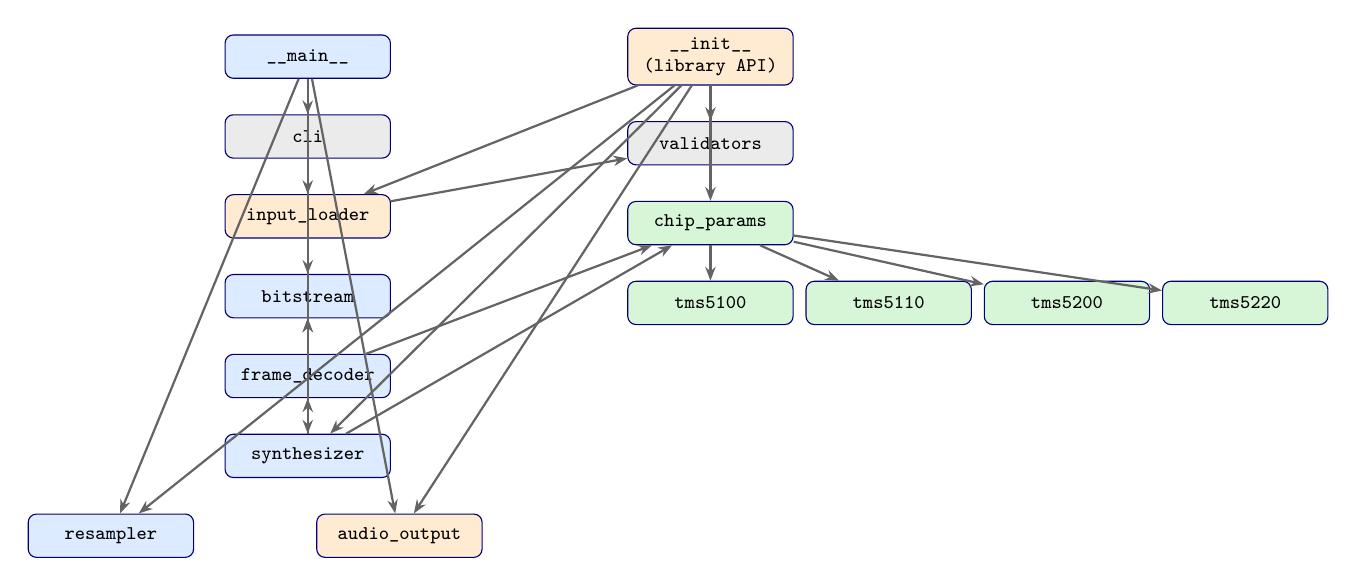
\begin{tikzpicture}[
  mod/.style={rectangle, rounded corners=3pt, draw=codeblue!70!black,
              fill=blockblue, minimum width=2.1cm, minimum height=0.55cm,
              font=\ttfamily\scriptsize, align=center},
  chip/.style={mod, fill=blockgreen},
  io/.style={mod, fill=blockorange},
  util/.style={mod, fill=blockgray},
  arr/.style={-{Stealth[length=5pt]}, draw=arrowgray, thick},
  node distance=0.55cm and 0.3cm,
]
% Row 0 — entry points
\node[mod] (main)   {\_\_main\_\_};
\node[io,  right=3.0cm of main] (init) {\_\_init\_\_\\(library API)};

% Row 1 — cli / validators
\node[util, below=0.45cm of main]  (cli)  {cli};
\node[util, below=0.45cm of init]  (val)  {validators};

% Row 2 — input_loader / chip_params
\node[io,   below=0.45cm of cli]   (inp)  {input\_loader};
\node[chip, below=0.45cm of val]   (cp)   {chip\_params};

% Row 3 — chips sub-package (right column) + bitstream (left column)
\node[chip, below=0.45cm of cp, xshift=0cm] (c100) {tms5100};
\node[chip, right=0.15cm of c100]              (c110) {tms5110};
\node[chip, right=0.15cm of c110]              (c200) {tms5200};
\node[chip, right=0.15cm of c200]              (c220) {tms5220};

% Row 4 — bitstream (left column, below inp, clear of chip row)
\node[mod, below=0.45cm of inp]  (bs)   {bitstream};

% Row 5 — frame_decoder
\node[mod, below=0.45cm of bs]  (fd)   {frame\_decoder};

% Row 6 — synthesizer
\node[mod, below=0.45cm of fd]  (syn)  {synthesizer};

% Row 7 — resampler / audio_output
\node[mod, below=0.45cm of syn, xshift=-2.5cm] (rs)   {resampler};
\node[io,  right=1.55cm of rs]                 (ao)   {audio\_output};

% Arrows
\draw[arr] (main) -- (cli);
\draw[arr] (main) -- (inp);
\draw[arr] (main) -- (syn);
\draw[arr] (main) -- (rs);
\draw[arr] (main) -- (ao);

\draw[arr] (init) -- (syn);
\draw[arr] (init) -- (rs);
\draw[arr] (init) -- (ao);
\draw[arr] (init) -- (inp);
\draw[arr] (init) -- (cp);
\draw[arr] (init) -- (val);

\draw[arr] (inp)  -- (val);
\draw[arr] (inp)  -- (bs);

\draw[arr] (cp)   -- (c100);
\draw[arr] (cp)   -- (c110);
\draw[arr] (cp)   -- (c200);
\draw[arr] (cp)   -- (c220);

\draw[arr] (fd)   -- (bs);
\draw[arr] (fd)   -- (cp);

\draw[arr] (syn)  -- (fd);
\draw[arr] (syn)  -- (bs);
\draw[arr] (syn)  -- (cp);
\end{tikzpicture}
\caption{Module dependency graph.  Blue~=~core pipeline;
  green~=~chip parameters; orange~=~I/O; grey~=~utilities.}
\label{fig:modules}
\end{figure}

\subsection{High-Level Data Flow}

Figure~\ref{fig:dataflow} illustrates the complete processing pipeline from
raw LPC bytes to a playable audio file.

% ── Data flow figure ─────────────────────────────────────────────────────────
\begin{figure}[H]
\centering
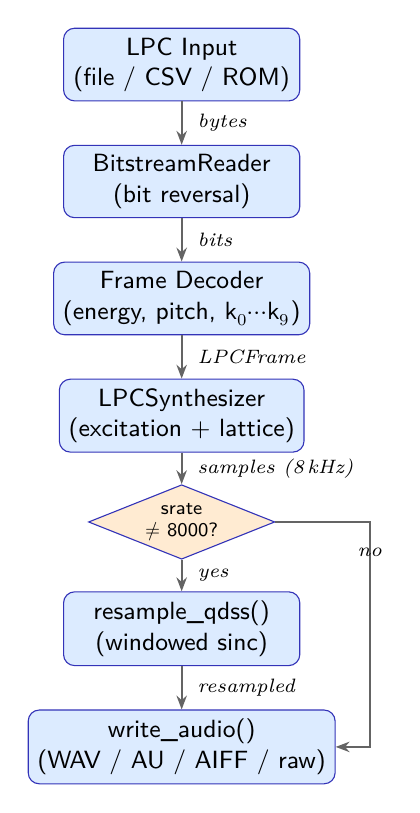
\begin{tikzpicture}[
  box/.style={rectangle, rounded corners=4pt, draw=codeblue!80,
              fill=blockblue, minimum width=3.0cm, minimum height=0.7cm,
              font=\small\sffamily, align=center},
  decision/.style={diamond, draw=codeblue!80, fill=blockorange,
                   font=\scriptsize\sffamily, align=center,
                   aspect=2.5, inner sep=1pt},
  arr/.style={-{Stealth[length=5pt]}, thick, draw=arrowgray},
  lab/.style={font=\scriptsize\itshape, midway, right=2pt},
  node distance=0.55cm,
]
\node[box]      (src)  {LPC Input\\(file / CSV / ROM)};
\node[box, below=of src]  (bs)   {BitstreamReader\\(bit reversal)};
\node[box, below=of bs]   (fd)   {Frame Decoder\\(energy, pitch, k$_0\!\cdots$k$_9$)};
\node[box, below=of fd]   (syn)  {LPCSynthesizer\\(excitation + lattice)};
\node[decision,below=0.4cm of syn] (srate) {srate\\$\neq$ 8000?};
\node[box, below=0.4cm of srate]  (rs)   {resample\_qdss()\\(windowed sinc)};
\node[box, below=of rs]   (ao)   {write\_audio()\\(WAV / AU / AIFF / raw)};

\draw[arr] (src)  -- (bs)   node[lab]{bytes};
\draw[arr] (bs)   -- (fd)   node[lab]{bits};
\draw[arr] (fd)   -- (syn)  node[lab]{LPCFrame};
\draw[arr] (syn)  -- (srate)node[lab]{samples (8\,kHz)};
\draw[arr] (srate)-- (rs)   node[lab]{yes};
% "no" path — skip resampler
\draw[arr] (srate.east) -| ++(1.2,0) |- (ao.east)
           node[pos=0.1, above, font=\scriptsize\itshape]{no};
\draw[arr] (rs)   -- (ao)   node[lab]{resampled};
\end{tikzpicture}
\caption{End-to-end data flow through \texttt{pyti\_lpc\_cmd}.}
\label{fig:dataflow}
\end{figure}

% ════════════════════════════════════════════════════════════════════════════
\section{LPC Bitstream Format}
\label{sec:bitstream}

\subsection{Bit Reversal}

Each byte in the LPC bitstream is stored in a bit-reversed order relative to
what the synthesizer expects.  Before any bits are extracted, each byte is
reversed in place using a three-stage swap network
(Figure~\ref{fig:bitreversal}).

\begin{equation}
\begin{aligned}
b &\leftarrow \bigl((b \gg 4) \mid (b \ll 4)\bigr) \;\&\; \texttt{0xFF}
  &&\text{(swap nibbles)} \\
b &\leftarrow \bigl(((b \;\&\; \texttt{0xCC}) \gg 2)
             \mid ((b \;\&\; \texttt{0x33}) \ll 2)\bigr) \;\&\; \texttt{0xFF}
  &&\text{(swap pairs)} \\
b &\leftarrow \bigl(((b \;\&\; \texttt{0xAA}) \gg 1)
             \mid ((b \;\&\; \texttt{0x55}) \ll 1)\bigr) \;\&\; \texttt{0xFF}
  &&\text{(swap bits)}
\end{aligned}
\label{eq:bitrev}
\end{equation}

% ── Bit reversal diagram ─────────────────────────────────────────────────────
\begin{figure}[H]
\centering
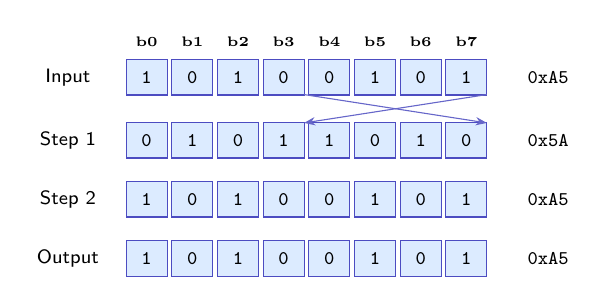
\begin{tikzpicture}[
  bit/.style={rectangle, draw=codeblue!70, fill=blockblue,
              minimum width=0.52cm, minimum height=0.45cm,
              font=\scriptsize\ttfamily},
  lbl/.style={font=\scriptsize\sffamily},
  arr/.style={-{Stealth[length=4pt]}, draw=arrowgray},
]
% Original byte  b7..b0 = 1 0 1 0 0 1 0 1  (0xA5)
\foreach \v/\i in {1/7,0/6,1/5,0/4,0/3,1/2,0/1,1/0}{
  \node[bit] at (\i*0.58, 2.1) {\v};
}
\node[lbl] at (-1.0, 2.1) {Input};
\node[lbl] at ( 5.1, 2.1) {\texttt{0xA5}};

% After step 1 (nibble swap): 0 1 0 1  1 0 1 0 = 0x5A
\foreach \v/\i in {0/7,1/6,0/5,1/4,1/3,0/2,1/1,0/0}{
  \node[bit] at (\i*0.58, 1.3) {\v};
}
\node[lbl] at (-1.0, 1.3) {Step 1};
\node[lbl] at ( 5.1, 1.3) {\texttt{0x5A}};

% After step 2 (pair swap): 1 0 1 0  0 1 0 1 = 0xA5
\foreach \v/\i in {1/7,0/6,1/5,0/4,0/3,1/2,0/1,1/0}{
  \node[bit] at (\i*0.58, 0.55) {\v};
}
\node[lbl] at (-1.0, 0.55) {Step 2};
\node[lbl] at ( 5.1, 0.55) {\texttt{0xA5}};

% After step 3 (bit swap): 1 0 1 0  0 1 0 1 → 0 1 0 1  1 0 1 0 = 0x5A? no: A5 is palindrome
\foreach \v/\i in {1/7,0/6,1/5,0/4,0/3,1/2,0/1,1/0}{
  \node[bit] at (\i*0.58, -0.2) {\v};
}
\node[lbl] at (-1.0,-0.2) {Output};
\node[lbl] at ( 5.1,-0.2) {\texttt{0xA5}};

% Bit position labels
\foreach \i in {0,...,7}{
  \node[font=\tiny\bfseries, black] at (\i*0.58, 2.55) {b\i};
}
% Arrows between rows for a couple of bits to show motion
\draw[arr,codeblue!60] (3*0.58+0.26, 2.1-0.22) -- (7*0.58+0.26, 1.3+0.22);
\draw[arr,codeblue!60] (7*0.58+0.26, 2.1-0.22) -- (3*0.58+0.26, 1.3+0.22);
\end{tikzpicture}
\caption{Three-stage bit reversal applied to \texttt{0xA5}.  Note that
  \texttt{0xA5} (\texttt{10100101}) is a bit palindrome and maps to itself.}
\label{fig:bitreversal}
\end{figure}

\subsection{Sliding-Window Bit Extraction}

After reversal, bits are extracted using a 16-bit sliding window spanning the
current and next bytes, left-shifted by the current bit offset, with the top
$N$ bits taken as the value (Figure~\ref{fig:sliding}).

\begin{figure}[H]
\centering
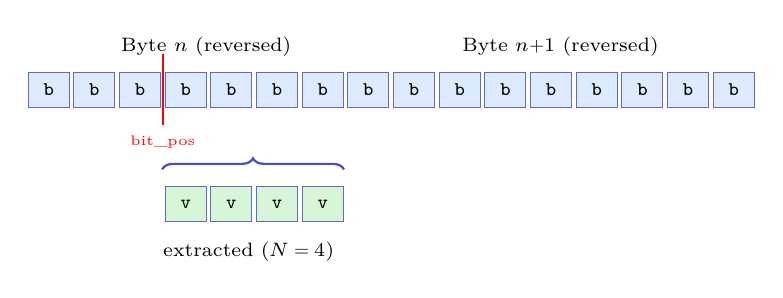
\begin{tikzpicture}[
  cell/.style={rectangle,draw=codeblue!60,fill=blockblue,
               minimum width=0.52cm,minimum height=0.45cm,
               font=\scriptsize\ttfamily},
  used/.style={cell,fill=blockgreen},
  span/.style={decorate,decoration={brace,amplitude=4pt},thick,draw=codeblue!70},
]
% Byte 0 (reversed) — top row
\foreach \i in {0,...,7}{
  \node[cell] at (\i*0.58+0.0, 0.9) {b};
}
% Byte 1 (reversed)
\foreach \i in {0,...,7}{
  \node[cell] at (\i*0.58+4.64, 0.9) {b};
}
% Row labels
\node[font=\scriptsize,black] at (2.0, 1.45) {Byte $n$ (reversed)};
\node[font=\scriptsize,black] at (6.5, 1.45) {Byte $n{+}1$ (reversed)};
% Bit offset marker — centered between 3rd and 4th b block (midpoint x=1.45)
\draw[red,thick] (1.45, 1.35) -- (1.45, 0.45)
    node[below,font=\tiny,red]{bit\_pos};
% Blue brace — halfway between old position and top of v blocks
\draw[span] (1.44, -0.11) -- (3.75, -0.11)
    node[midway,below=3pt,font=\scriptsize]{};
% Extracted bit blocks
\foreach \i in {3,4,5,6}{
  \node[used] at (\i*0.58, -0.55) {v};
}
% "extracted" label: left edge aligned with left side of first v block (x=1.48)
\node[font=\scriptsize, anchor=west] at (1.33, -1.15) {extracted ($N=4$)};
\end{tikzpicture}
\caption{Sliding-window extraction of $N=4$ bits starting at \texttt{bit\_pos}=3
  within byte $n$.}
\label{fig:sliding}
\end{figure}

\subsection{Frame Structure}

Figure~\ref{fig:frameformat} shows the variable-width bit field layout for the
three frame types.  A data frame for a voiced sound with new coefficients
consumes up to $4+1+6+5+5+4+4+4+4+4+3+3+3 = 54$ bits on a 6-bit pitch chip.

\begin{figure}[H]
\centering
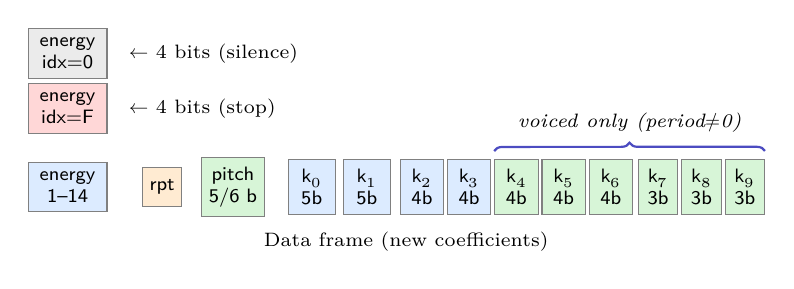
\begin{tikzpicture}[
  fld/.style={rectangle,draw=gray,fill=blockblue,
              minimum height=0.5cm,font=\scriptsize\sffamily,
              inner xsep=2pt,align=center},
  sil/.style={fld,fill=blockgray},
  stop/.style={fld,fill=blockred},
  vo/.style={fld,fill=blockgreen},
  rep/.style={fld,fill=blockorange},
]
% Silence frame
\node[sil, minimum width=1.0cm] (e0) at (0,2.2) {energy\\idx=0};
\node[font=\scriptsize,black,right=0.15cm of e0] {$\leftarrow$ 4 bits (silence)};

% Stop frame
\node[stop, minimum width=1.0cm] (ef) at (0,1.5) {energy\\idx=F};
\node[font=\scriptsize,black,right=0.15cm of ef] {$\leftarrow$ 4 bits (stop)};

% Data frame (voiced, new coefficients)
\node[fld,  minimum width=1.0cm] (en)  at (0.0, 0.5) {energy\\1--14};
\node[rep,  minimum width=0.5cm] (rpt) at (1.2, 0.5) {rpt};
\node[vo,   minimum width=0.8cm] (pit) at (2.1, 0.5) {pitch\\5/6 b};
\node[fld,  minimum width=0.6cm] (k0)  at (3.1, 0.5) {k$_0$\\5b};
\node[fld,  minimum width=0.6cm] (k1)  at (3.8, 0.5) {k$_1$\\5b};
\node[fld,  minimum width=0.55cm](k2)  at (4.5, 0.5) {k$_2$\\4b};
\node[fld,  minimum width=0.55cm](k3)  at (5.1, 0.5) {k$_3$\\4b};
\node[vo,   minimum width=0.55cm](k4)  at (5.7, 0.5) {k$_4$\\4b};
\node[vo,   minimum width=0.55cm](k5)  at (6.3, 0.5) {k$_5$\\4b};
\node[vo,   minimum width=0.55cm](k6)  at (6.9, 0.5) {k$_6$\\4b};
\node[vo,   minimum width=0.5cm] (k7)  at (7.5, 0.5) {k$_7$\\3b};
\node[vo,   minimum width=0.5cm] (k8)  at (8.05,0.5) {k$_8$\\3b};
\node[vo,   minimum width=0.5cm] (k9)  at (8.6, 0.5) {k$_9$\\3b};

% Brace for voiced-only
\draw[decorate,decoration={brace,amplitude=3pt,raise=3pt},thick,draw=codeblue!70]
    (k4.north west) -- (k9.north east)
    node[midway,above=6pt,font=\scriptsize\itshape]{voiced only (period$\neq$0)};

\node[font=\scriptsize,black] at (4.3,-0.2) {Data frame (new coefficients)};
\end{tikzpicture}
\caption{LPC frame bit-field layouts.  Green fields are voiced-only; orange
  is the repeat flag.  When \texttt{repeat}=1, k-coefficient fields are
  absent and the previous values are reused.}
\label{fig:frameformat}
\end{figure}

% ════════════════════════════════════════════════════════════════════════════
\section{LPC Synthesis Engine}
\label{sec:synth}

\subsection{Frame Timing and Interpolation}

Each LPC frame spans 25~ms at the native 8\,kHz rate, yielding exactly 200
samples per frame.  To avoid abrupt parameter changes at frame boundaries, the
synthesizer linearly interpolates energy, pitch, and all ten reflection
coefficients across eight equally-spaced sub-steps of 25 samples each.

The interpolation uses an arithmetic right-shift approximation:

\begin{equation}
c_{\mathrm{cur}} \leftarrow c_{\mathrm{cur}} +
  \left\lfloor \frac{c_{\mathrm{tgt}} - c_{\mathrm{cur}}}{2^{s_i}}
  \right\rfloor
\label{eq:interp}
\end{equation}

where $s_i$ is the shift for sub-step $i$ from the sequence
$\mathbf{s} = [0, 3, 3, 3, 2, 2, 1, 1]$.  A shift of~0 at step~0 means no
change; by step~7 (shift~1) the parameter moves halfway toward the target.

Figure~\ref{fig:interp} illustrates the interpolation trajectory for a single
parameter transitioning from value 100 to 200.

\begin{figure}[H]
\centering
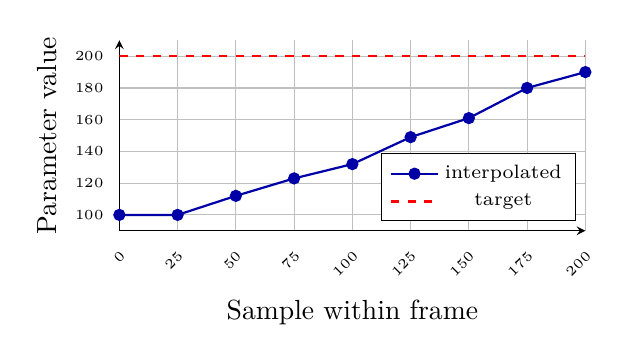
\begin{tikzpicture}
\begin{axis}[
  width=7.5cm, height=4.0cm,
  xlabel={Sample within frame},
  ylabel={Parameter value},
  xmin=0, xmax=200,
  ymin=90, ymax=210,
  xtick={0,25,50,75,100,125,150,175,200},
  xticklabel style={font=\tiny,rotate=45,anchor=north east},
  ytick={100,120,140,160,180,200},
  yticklabel style={font=\tiny},
  grid=both,
  grid style={line width=0.3pt,draw=gray!30},
  major grid style={line width=0.4pt,draw=gray!50},
  tick style={draw=none},
  axis lines=left,
  legend style={font=\scriptsize,at={(0.98,0.05)},anchor=south east},
]
% Shifts: [0,3,3,3,2,2,1,1]  start=100 target=200
% s0=0: no change -> 100
% s25: shift3: 100+(100>>3)=100+12=112
% s50: shift3: 112+(88>>3)=112+11=123
% s75: shift3: 123+(77>>3)=123+9=132
% s100:shift2: 132+(68>>2)=132+17=149
% s125:shift2: 149+(51>>2)=149+12=161
% s150:shift1: 161+(39>>1)=161+19=180
% s175:shift1: 180+(20>>1)=180+10=190
\addplot[codeblue,thick,mark=*,mark size=1.8pt] coordinates {
  (0,100)(25,100)(50,112)(75,123)(100,132)(125,149)(150,161)(175,180)(200,190)
};
\addplot[red,dashed,thick] coordinates {(0,200)(200,200)};
\legend{interpolated,target}
\end{axis}
\end{tikzpicture}
\caption{Interpolation trajectory for a parameter stepping from 100 to~200
  using the shift sequence $[0,3,3,3,2,2,1,1]$.  The value converges
  toward (but does not reach) the target within one frame.}
\label{fig:interp}
\end{figure}

Interpolation is \emph{skipped} (parameters jump directly to target) at
transitions between silence and sound, and between voiced and unvoiced
excitation, to prevent audible transient artefacts.

\subsection{Excitation Generation}

The LPC model separates the vocal tract (lattice filter) from the excitation
source~\cite{Rabiner1978,Atal1971}.  Two sources are used depending on the pitch period parameter.

\paragraph{Voiced excitation (period~$> 0$).}
A chirp waveform stored in the chip's ROM is played repeatedly at the pitch
period.  The chirp is an empirically-derived impulse response that
approximates glottal closure.  Only the first 41 samples of the chirp table
produce non-zero values; beyond that the excitation is zero.

\begin{equation}
u_{10} = \frac{\text{int8}(\mathrm{chirp}[p])}
              {256} \;\cdot\; \frac{E}{256}
\label{eq:voiced_exc}
\end{equation}

where $p$ is the period counter ($0 \le p < P$, cycling at period $P$), $E$
is the energy parameter, and the chirp value is reinterpreted from unsigned
uint8 to signed int8 before use.

\paragraph{Unvoiced excitation (period~$= 0$).}
A 16-bit Galois LFSR generates pseudo-random noise:

\begin{equation}
r \leftarrow (r \gg 1) \;\oplus\; \begin{cases}
  \texttt{0xB800} & \text{if } r \;\&\; 1 \\
  0               & \text{otherwise}
\end{cases},
\quad u_{10} = \frac{\pm E}{2048}
\label{eq:lfsr}
\end{equation}

The sign of the excitation follows the new LSB of $r$.  The LFSR is reset to
1 at the start of each utterance, ensuring bit-exact reproducibility.

\subsection{10th-Order Lattice Filter}
\label{sec:lattice}

The vocal tract is modeled as a series of ten coupled acoustic tube sections,
implemented as a lattice (ladder) filter.  The filter maintains ten delay
states $\mathbf{x} = [x_0, x_1, \ldots, x_9]$, all initialised to zero.

The reflection coefficients $k_0 \cdots k_9$ are stored in the chip parameter
tables as scaled integers; the true coefficient is $k_n / 512$.

Figure~\ref{fig:lattice} shows the signal flow graph for one filter stage.

% ── Lattice filter figure ────────────────────────────────────────────────────
\begin{figure}[H]
\centering
\begin{tikzpicture}[
  sum/.style={circle,draw=codeblue!70,fill=white,
              minimum size=0.45cm,inner sep=0pt,font=\small},
  delay/.style={rectangle,draw=gray,fill=blockgray,
                minimum width=0.7cm,minimum height=0.45cm,
                font=\scriptsize\ttfamily},
  mult/.style={draw=codeblue!70,fill=blockblue,
               regular polygon,regular polygon sides=3,shape border rotate=0,
               minimum size=0.5cm,inner sep=0pt,font=\scriptsize},
  arr/.style={-{Stealth[length=4.5pt]},thick,draw=arrowgray},
  node distance=0.7cm,
]

%% Forward path: u_{n+1} → sa → z^{-1} → sb → u_n
\node[sum]   (sa)  at (0,   0) {$+$};
\node[sum]   (sb)  at (5.1, 0) {$+$};

% Inputs
\node[font=\small] (un1) at (-2.2, 0) {$u_{n+1}$};
\node[font=\small] (un)  at (7.8,  0) {$u_n$};

% Delay state
\node[delay] (xn)  at (3.0, 0) {$z^{-1}$};
\node[font=\scriptsize] (xnlbl) at (4.3, 0.3) {$x_n$};

% Coefficient labels (spread further vertically)
\node[font=\scriptsize,codeblue] (kn_f) at (3.0,  3.2) {$-k_n/512$};
\node[font=\scriptsize,codeblue] (kn_r) at (3.0, -2.4) {$+k_n/512$};

% Arrows — forward path
\draw[arr] (un1) -- (sa);
\draw[arr] (sa)  -- (xn);
\draw[arr] (xn)  -- (sb);
\draw[arr] (sb)  -- (un);

% Feedback top: xn up 2.0 cm then left to sa (−kn/512)
\draw[arr,codeblue!60] (xn.north) -- ++(0,2.0)
    -| node[pos=0.08,above,font=\scriptsize]{$\times(-k_n/512)$} (sa.north);

% Feedback bottom: xn down 1.4 cm then right to sb (+kn/512)
\draw[arr,codeblue!60] (xn.south) -- ++(0,-1.4)
    -| node[pos=0.08,below,font=\scriptsize]{$\times(+k_n/512)$} (sb.south);

%% Reverse path: goes 3.5 cm below main path — well clear of +kn/512 path
\draw[arr,red!70,dashed] (sa.south) -- ++(0,-3.5) -| (sb.south);
\node[font=\scriptsize\itshape,red!70] at (3.0, -4.1) {update $x_n$};

\end{tikzpicture}
\caption{Signal flow for one stage ($n$) of the 10th-order lattice filter.
  \textbf{Black} solid arrows carry the forward signal path computing $u_n$.
  \textbf{Blue} paths show the coefficient feedback ($\times k_n/512$) from
  the delay state $x_n$ to each summing node.
  The \textbf{red} dashed path marks the reverse (feedback-update) path that
  refreshes the delay state $x_n$ after each sample.}
\label{fig:lattice}
\end{figure}

\paragraph{Forward path.}  The excitation $u_{10}$ enters stage 9 and
propagates to stage 0:

\begin{align}
u_m &= u_{m+1} - \frac{k_m}{512}\, x_m, \quad m = 9, 8, \ldots, 0
\label{eq:forward}
\end{align}

The final output $u_0$ is clamped to $[-1, 1]$ to prevent filter runaway.

\paragraph{Reverse path.}  Delay states are updated using the forward-path
intermediate values:

\begin{align}
x_m &= x_{m-1} + \frac{k_{m-1}}{512}\, u_{m-1}, \quad m = 9, 8, \ldots, 1 \nonumber\\
x_0 &= u_0
\label{eq:reverse}
\end{align}

The final output sample is $u_0 \times 1.5$ (an empirical post-filter gain
stage replicating the original chip's output level).

Figure~\ref{fig:lattice_full} shows the complete 10-stage cascade.

% ── Full 10-stage lattice ─────────────────────────────────────────────────────
\begin{figure}[t]
\centering
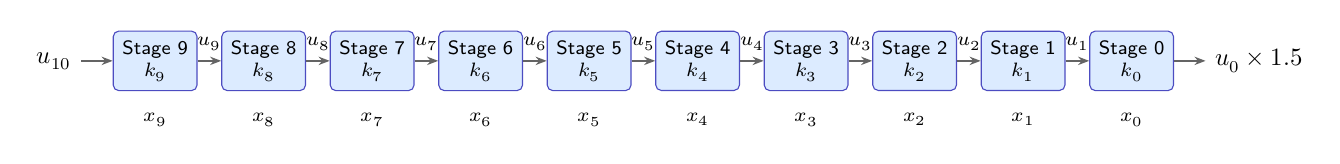
\begin{tikzpicture}[
  stg/.style={rectangle,rounded corners=2pt,draw=codeblue!70,fill=blockblue,
              minimum width=1.0cm,minimum height=0.55cm,
              font=\scriptsize\sffamily,align=center},
  arr/.style={-{Stealth[length=4pt]},thick,draw=arrowgray},
  node distance=0.1cm and 0.3cm,
]
\node[stg] (s9) {Stage 9\\$k_9$};
\node[stg,right=0.3cm of s9] (s8) {Stage 8\\$k_8$};
\node[stg,right=0.3cm of s8] (s7) {Stage 7\\$k_7$};
\node[stg,right=0.3cm of s7] (s6) {Stage 6\\$k_6$};
\node[stg,right=0.3cm of s6] (s5) {Stage 5\\$k_5$};
\node[stg,right=0.3cm of s5] (s4) {Stage 4\\$k_4$};
\node[stg,right=0.3cm of s4] (s3) {Stage 3\\$k_3$};
\node[stg,right=0.3cm of s3] (s2) {Stage 2\\$k_2$};
\node[stg,right=0.3cm of s2] (s1) {Stage 1\\$k_1$};
\node[stg,right=0.3cm of s1] (s0) {Stage 0\\$k_0$};

\node[left=0.4cm of s9,font=\small\sffamily] (u10) {$u_{10}$};
\node[right=0.4cm of s0,font=\small\sffamily] (out) {$u_0\times 1.5$};

\draw[arr] (u10) -- (s9);
\draw[arr] (s9)  -- (s8) node[midway,above,font=\scriptsize]{$u_9$};
\draw[arr] (s8)  -- (s7) node[midway,above,font=\scriptsize]{$u_8$};
\draw[arr] (s7)  -- (s6) node[midway,above,font=\scriptsize]{$u_7$};
\draw[arr] (s6)  -- (s5) node[midway,above,font=\scriptsize]{$u_6$};
\draw[arr] (s5)  -- (s4) node[midway,above,font=\scriptsize]{$u_5$};
\draw[arr] (s4)  -- (s3) node[midway,above,font=\scriptsize]{$u_4$};
\draw[arr] (s3)  -- (s2) node[midway,above,font=\scriptsize]{$u_3$};
\draw[arr] (s2)  -- (s1) node[midway,above,font=\scriptsize]{$u_2$};
\draw[arr] (s1)  -- (s0) node[midway,above,font=\scriptsize]{$u_1$};
\draw[arr] (s0)  -- (out);

% Delay states below
\foreach \s/\n in {s9/9,s8/8,s7/7,s6/6,s5/5,s4/4,s3/3,s2/2,s1/1,s0/0}{
  \node[font=\scriptsize\ttfamily,black,below=0.15cm of \s]{$x_{\n}$};
}
\end{tikzpicture}
\caption{Complete 10-stage lattice filter cascade.  Excitation $u_{10}$ enters
  stage~9; each stage applies its reflection coefficient $k_m$ and delay
  state $x_m$ to produce intermediate signal $u_m$.  Output is $u_0\times 1.5$.}
\label{fig:lattice_full}
\end{figure}

% ════════════════════════════════════════════════════════════════════════════
\FloatBarrier
\section{Sample Rate Conversion}
\label{sec:src}

The synthesizer produces samples natively at 8\,kHz.  When a different output
rate is requested, a windowed-sinc FIR resampler (QDSS algorithm, R.\,H.\,Nicholson~Jr.~\cite{Nicholson_QDSS}) converts the sample rate.

For each output sample at fractional position $x$ in the input buffer:

\begin{equation}
y = G \sum_{j=\lfloor x\rfloor - W/2}^{\lfloor x\rfloor + W/2}
    w(j-x,W)\;\cdot\;\mathrm{sinc}\!\left(\frac{2\pi(j-x)f_{\max}}{f_s}\right)
    \cdot \mathrm{input}[j]
\label{eq:qdss}
\end{equation}

where $G = 2f_{\max}/f_s$, and $w(\cdot)$ is the von~Hann window:

\begin{equation}
w(\delta, W) = \tfrac{1}{2} - \tfrac{1}{2}
  \cos\!\left(2\pi\!\left(\tfrac{1}{2} + \tfrac{\delta}{W}\right)\right)
\label{eq:hann}
\end{equation}

Filter parameters are chosen to balance quality against computation:

\begin{center}
\begin{tabular}{lll}
\toprule
Direction    & $f_{\max}$            & Window width $W$ \\
\midrule
Upsampling   & $f_{\mathrm{out}} \times 0.55$  & 64   \\
Downsampling & $f_{\mathrm{out}} \times 0.375$ & 256  \\
\bottomrule
\end{tabular}
\end{center}

% ════════════════════════════════════════════════════════════════════════════
\section{Audio Output}
\label{sec:audio}

The \texttt{audio\_output} module writes four file formats, detected
automatically from the output file extension.  For WAV files, the RIFF chunk
structure is generated entirely in Python using \texttt{struct.pack}; no
third-party libraries are required.

\paragraph{PCM encoding.}
Float samples in $[-1.0, 1.0]$ are converted to integers after applying the
user-specified gain ($G \in [0, 3]$, default 0.90):

\[
\text{int\_val} = \text{round}(s \cdot G \cdot \text{peak})
\]

where peak~$= 32767$ for 16-bit and peak~$= 127$ for 8-bit. Eight-bit WAV uses
unsigned encoding with a centre offset of~128.

\paragraph{Channel routing.}
Stereo output places the synthesised signal on both channels by default; the
\texttt{ch=left}, \texttt{ch=right} options route audio to one channel with
silence on the other.

% ════════════════════════════════════════════════════════════════════════════
\section{Input Formats and Validation}
\label{sec:input}

Six mutually exclusive input sources are supported:

\begin{enumerate}[noitemsep]
\item \textbf{strbin=} — raw binary LPC file (max 32\,KB)
\item \textbf{str=} — decimal CSV string, optional \texttt{label:} prefix
\item \textbf{strhex=} — hex CSV string, optional \texttt{0x} prefixes
\item \textbf{strfile=} — decimal CSV text file (max 1\,MB)
\item \textbf{strhexfile=} — hex CSV text file (max 1\,MB)
\item \textbf{addr=} — address within a VSM ROM file
\end{enumerate}

All string inputs are validated character-by-character against a whitelist
before parsing.  File paths are checked for directory traversal sequences
(\texttt{..}).  Buffer sizes are bounded at file-load time.

% ════════════════════════════════════════════════════════════════════════════
\section{Chip Variants and Parameter Tables}
\label{sec:chips}

Each chip variant is characterised by a set of lookup tables that map compact
bitstream indices to physical parameter values.  All four variants have the
same ten coefficient tables ($k_0$--$k_9$) but differ in their chirp waveform,
energy table, pitch table, and pitch counter width.

\begin{center}
\begin{tabular}{lllll}
\toprule
Chip    & Pitch & Entries & Chirp & Energy \\
\midrule
TMS5100 & 5-bit & 32 & 50-entry decimal & 16-entry \\
TMS5110 & 5-bit & 32 & 32-entry decimal & 16-entry \\
TMS5200 & 6-bit & 64 & 52-entry hex     & 16-entry \\
TMS5220 & 6-bit & 64 & 52-entry hex     & 16-entry \\
\bottomrule
\end{tabular}
\end{center}

The TMS5220 energy table is
$\{0, 1, 2, 3, 4, 6, 8, 11, 16, 23, 33, 47, 63, 85, 114, 0\}$; note that
index~15 maps to 0, which combined with the preceding \texttt{is\_stop} flag
makes energy effectively 0 during drain frames.

Tables are embedded directly in the \texttt{chips/} sub-package, making the
package self-contained without requiring external data files~\cite{TMS5220_1983,TMS5100_1981}.

% ════════════════════════════════════════════════════════════════════════════
\section{Verification}
\label{sec:verify}

The reference test vector from the specification is the 223-byte file
\texttt{0220\_Affirmative.lpc} (TMS5220 encoding of the word ``affirmative'').
The expected output properties are summarised in Table~\ref{tab:verify}.

\begin{table}[H]
\centering
\caption{Reference test vector verification results.}
\label{tab:verify}
\begin{tabular}{lll}
\toprule
Property             & Expected & Result  \\
\midrule
Frames decoded       & 35 (33 + 2 drain) & $\checkmark$\\
Total samples        & 7000    & $\checkmark$\\
Stereo 16-bit WAV    & 28044 B & $\checkmark$\\
Mono 16-bit WAV      & 14044 B & $\checkmark$\\
Mono 8-bit WAV       & 7044 B  & $\checkmark$\\
Stop + drain samples & 400     & $\checkmark$\\
Loop guard (200 fr.\ = 5 s) & 40000 B & $\checkmark$\\
\bottomrule
\end{tabular}
\end{table}

% ════════════════════════════════════════════════════════════════════════════
\section{Security Considerations}
\label{sec:security}

The implementation follows defensive input handling throughout:

\begin{itemize}[noitemsep]
\item All string inputs are validated against character whitelists before
  integer parsing.
\item File sizes are bounded before reading (1\,MB text, 32\,KB binary LPC,
  16\,KB per ROM slot).
\item File paths are checked for traversal sequences (\texttt{..}).
\item The bitstream reader returns 0 for reads past the buffer end, preventing
  index-out-of-bounds on malformed inputs.
\item The lattice filter output is clamped to $[-1.0, 1.0]$ after every
  sample, preventing NaN/Inf propagation through the pipeline.
\item The infinite-loop guard (default 200 frames = 5 seconds at 8\,kHz)
  bounds execution time on silence-only inputs.
\end{itemize}

% ════════════════════════════════════════════════════════════════════════════
\section{Conclusion}
\label{sec:conclusion}

\texttt{pyti\_lpc\_cmd} is a complete, clean-room Python implementation of the
TMS5xxx LPC speech decoder.  The implementation faithfully reproduces the
bitstream format, excitation model, lattice filter, and interpolation behavior
of the original hardware, verified against known-good reference output.  The
package is designed for both standalone command-line use and embedding as a
library in Python applications.

% ════════════════════════════════════════════════════════════════════════════
% ── Appendix ─────────────────────────────────────────────────────────────────
% ════════════════════════════════════════════════════════════════════════════
\clearpage
\appendix
\appendixpage

\section{Python Library Interface Reference}
\label{app:libapi}

This appendix documents the complete public API exposed when
\texttt{pyti\_lpc\_cmd} is imported as a Python library.  All symbols listed
here are accessible after \lstinline{import pyti_lpc_cmd as lpc} and are
enumerated in the package's \texttt{\_\_all\_\_} list.

\subsection{High-Level Interface}

\subsubsection{\texttt{render()} — One-Call Pipeline}

\begin{lstlisting}[caption={render() function signature}]
samples = lpc.render(
    data       : bytes,
    chip       : str  = "tms5220",
    *,
    srate      : int  = 8000,
    swidth     : int  = 16,
    gain       : int  = 90,
    output     : str  = "stereo",
    ch         : str  = "both",
    wav        : str  = None,
    use_interp : bool = True,
    use_filter : bool = True,
    max_frames : int  = 200,
    use_loopguard : bool = True,
    verbose    : bool = False,
) -> list[float]
\end{lstlisting}

\noindent Decodes an LPC bitstream and optionally writes an audio file.
Returns a \texttt{list[float]} of samples at \texttt{srate}~Hz.

\begin{center}
\begin{tabular}{p{2.6cm}>{\raggedright\arraybackslash}p{9.5cm}}
\toprule
Parameter & Description \\
\midrule
\texttt{data}       & Raw LPC bitstream bytes. \\
\texttt{chip}       & Chip name (\texttt{"tms5100"}, \texttt{"tms5110"},
                      \texttt{"tms5200"}, \texttt{"tms5220"}) or path to a
                      \texttt{.txt} chip definition file. \\
\texttt{srate}      & Output sample rate in Hz.  Values other than 8000
                      trigger windowed-sinc resampling. \\
\texttt{swidth}     & Bits per sample for file output: \texttt{8} or
                      \texttt{16}. \\
\texttt{gain}       & Gain percentage 0--300.  Default 90 maps to $\times 0.90$
                      before integer conversion. \\
\texttt{output}     & \texttt{"stereo"}/\texttt{"st"} or
                      \texttt{"mono"}/\texttt{"mo"}. \\
\texttt{ch}         & For stereo: \texttt{"both"} (default),
                      \texttt{"left"}/\texttt{"l"}/\texttt{"0"}, or
                      \texttt{"right"}/\texttt{"r"}/\texttt{"1"}. \\
\texttt{wav}        & Output file path.  Extension determines format.
                      \texttt{None} = no file written. \\
\texttt{use\_interp}& Enable parameter interpolation (default
                      \texttt{True}). \\
\texttt{use\_filter}& Enable the lattice filter.  \texttt{False} produces
                      silence (useful for testing). \\
\texttt{max\_frames}& Infinite-loop guard: halt after this many consecutive
                      silence frames (default 200 = 5 seconds at 8\,kHz). \\
\texttt{use\_loopguard}& Enable the infinite-loop guard (default \texttt{True}).
                      Pass \texttt{False} to disable. \\
\texttt{verbose}    & Print per-frame diagnostic lines to stdout. \\
\bottomrule
\end{tabular}
\end{center}

\medskip\noindent\textbf{Example usage.}\par\vspace{4pt}
\begin{lstlisting}[caption={Common render() patterns}]
import pyti_lpc_cmd as lpc

# Render to WAV, get samples back
with open("word.lpc", "rb") as f:
    data = f.read()

samples = lpc.render(data, chip="tms5220",
                     wav="out.wav")

# Mono 44.1 kHz 16-bit
lpc.render(data, chip="tms5220",
           wav="out_44k.wav",
           srate=44100, output="mono")

# Raw float samples only (no file)
samples = lpc.render(data, chip="tms5220")

# From hex CSV inline
data = lpc.load_hex_csv("A5,4F,7A,D3,3C,5A")
samples = lpc.render(data, chip="tms5220",
                     wav="snippet.au")
\end{lstlisting}

\subsection{Chip Management}

\subsubsection{\texttt{get\_builtin\_chip(name)}}

Returns a \texttt{ChipParams} instance for one of the four built-in chip
variants.

\begin{lstlisting}
chip = lpc.get_builtin_chip("tms5220")
# Accepted: "tms5100", "tms5110", "tms5200", "tms5220"
# Also accepts names with ".txt" suffix stripped.
\end{lstlisting}

\subsubsection{\texttt{load\_chip\_file(path)}}

Parses a plain-text chip definition file and returns a \texttt{ChipParams}
instance.

\begin{lstlisting}
chip = lpc.load_chip_file("/data/custom_chip.txt")
\end{lstlisting}

\subsubsection{\texttt{ChipParams} dataclass}

\begin{lstlisting}
@dataclass
class ChipParams:
    processor   : str
    chirp       : list[int]   # uint8, len 32/50/52
    energy      : list[int]   # 16 entries
    pitch_count : int          # 32 or 64
    pitch       : list[int]   # pitch period table
    k0 .. k9    : list[int]   # reflection coeff x512
\end{lstlisting}

The \texttt{k\_table(n)} method returns the coefficient table for index $n$
(0--9).

\subsection{Synthesis Pipeline}

\needspace{6\baselineskip}
\subsubsection{\texttt{LPCSynthesizer}}

\begin{lstlisting}[caption={Mid-level synthesis}]
chip   = lpc.get_builtin_chip("tms5220")
synth  = lpc.LPCSynthesizer()
samples = synth.synthesize(
    data,
    chip,
    use_interp = True,
    max_frames = 200,
    verbose    = False,
)  # -> list[float] at 8000 Hz
\end{lstlisting}

State (delay registers, LFSR seed, period counter) is reset automatically at
the start of each \texttt{synthesize()} call.

\subsubsection{\texttt{BitstreamReader}}

\begin{lstlisting}[caption={Low-level bitstream access}]
reader = lpc.BitstreamReader(data, reverse_bits=True)
energy_idx = reader.get_bits(4)   # read 4 bits
repeat     = reader.get_bits(1)   # read 1 bit
pitch_idx  = reader.get_bits(6)   # read 6 bits

# Static helper
rev = lpc.BitstreamReader.reverse_byte(0xA5)  # 0xA5
\end{lstlisting}

\subsubsection{\texttt{LPCFrame} and \texttt{decode\_frame()}}

\begin{lstlisting}[caption={Frame-by-frame decoding loop}]
prev_k = [0] * 10
reader = lpc.BitstreamReader(data)

while True:
    frame = lpc.decode_frame(reader,
                             chip, prev_k)
    if frame.is_stop:
        break
    if not frame.is_silence:
        # frame.energy, frame.period,
        # frame.repeat, frame.k[0..9]
        prev_k = list(frame.k)
\end{lstlisting}

\subsubsection{\texttt{resample\_qdss(input\_buf, input\_rate, output\_rate)}}

\begin{lstlisting}
resampled = lpc.resample_qdss(
    samples, 8000.0, 44100.0
)
\end{lstlisting}

Returns identity (shallow copy) when rates are equal.

\subsection{Audio Output}

All write functions accept float samples in $[-1.0, 1.0]$.  The
\texttt{gain} argument is a multiplier (e.g. \texttt{0.75} for 75\%).

\begin{lstlisting}[caption={Audio output functions}]
# Auto-detect format from extension
lpc.write_audio("out.wav",  ch0, ch1,
                srate, bits, channels, gain)

# Explicit format
lpc.write_wav( "out.wav",  ch0, ch1,
               srate, bits, channels, gain)
lpc.write_au(  "out.au",   ch0, ch1,
               srate, bits, channels, gain)
lpc.write_aiff("out.aiff", ch0, ch1,
               srate, bits, channels, gain)
lpc.write_raw( "out.raw",  ch0, ch1,
               bits, channels, gain)
\end{lstlisting}

\noindent For mono output, pass \texttt{ch1=None} and \texttt{channels=1}.

\subsection{Input Loaders}

\begin{lstlisting}[caption={Input loader functions}]
# Binary file  (max 32 KB)
data = lpc.load_binary_file("word.lpc")

# Decimal CSV - optional label prefix
data = lpc.load_decimal_csv("isle:165,79,122")

# Decimal CSV from text file  (max 1 MB)
data = lpc.load_decimal_csv_file("input.txt")

# Hex CSV - optional 0x prefix
data = lpc.load_hex_csv("A5,4F,0x7A,D3")

# Hex CSV from text file
data = lpc.load_hex_csv_file("input.txt")

# ROM operations
rom  = lpc.load_rom_file("speak_spell.bin")
data = lpc.load_rom_address(rom, 0x0220)

# Combine two ROM slots into 32 KB flat space
full = lpc.build_rom(rom0_bytes, rom1_bytes)
\end{lstlisting}

\subsection{Validation Utilities}

\begin{lstlisting}[caption={Input validation}]
try:
    lpc.validate_decimal_string(s)
    lpc.validate_hex_string(s)
    lpc.validate_file_path(path)
except lpc.ValidationError as e:
    print("Bad input:", e)
\end{lstlisting}

\texttt{ValidationError} is a subclass of \texttt{ValueError}.

\subsection{Complete \texttt{\_\_all\_\_} Reference}

\begin{center}
\begin{tabular}{ll}
\toprule
Symbol & Category \\
\midrule
\texttt{render}              & High-level pipeline \\
\texttt{ChipParams}          & Chip management \\
\texttt{get\_builtin\_chip}  & Chip management \\
\texttt{load\_chip\_file}    & Chip management \\
\texttt{LPCSynthesizer}      & Synthesis \\
\texttt{LPCFrame}            & Synthesis \\
\texttt{BitstreamReader}     & Synthesis \\
\texttt{decode\_frame}       & Synthesis \\
\texttt{resample\_qdss}      & Resampling \\
\texttt{write\_wav}          & Audio output \\
\texttt{write\_au}           & Audio output \\
\texttt{write\_aiff}         & Audio output \\
\texttt{write\_raw}          & Audio output \\
\texttt{write\_audio}        & Audio output \\
\texttt{load\_binary\_file}  & Input loading \\
\texttt{load\_decimal\_csv}  & Input loading \\
\texttt{load\_decimal\_csv\_file} & Input loading \\
\texttt{load\_hex\_csv}      & Input loading \\
\texttt{load\_hex\_csv\_file}& Input loading \\
\texttt{load\_rom\_file}     & Input loading \\
\texttt{load\_rom\_address}  & Input loading \\
\texttt{build\_rom}          & Input loading \\
\texttt{strip\_label\_prefix}& Input loading \\
\texttt{ValidationError}     & Validation \\
\texttt{validate\_decimal\_string} & Validation \\
\texttt{validate\_hex\_string} & Validation \\
\texttt{validate\_file\_path} & Validation \\
\bottomrule
\end{tabular}
\end{center}

\clearpage
\section{Command-Line Interface Reference}
\label{app:cli}

The \texttt{\_\_main\_\_} module is invoked as
\texttt{python~-m~pyti\_lpc\_cmd~[key=value~\ldots]}.
All parameters use the \texttt{key=value} form; order is irrelevant.

\subsection{CLI Parameters}

\begin{center}
\begin{tabular}{p{2.8cm}p{2.1cm}>{\raggedright\arraybackslash}p{7.4cm}}
\toprule
Parameter & Default & Description \\
\midrule
\texttt{mode=}      & ---    & Operation mode: \texttt{render}, \texttt{romlist},
                               \texttt{rendaddrfileseq}, \texttt{rendstrfileseq},
                               \texttt{cleanbrace}, \texttt{cleanquote}. \\
\texttt{chip=}      & \texttt{tms5220} & Built-in chip name or path to a
                               \texttt{.txt} chip definition file. \\
\texttt{strbin=}    & ---    & Path to a raw binary LPC file. \\
\texttt{str=}       & ---    & Decimal CSV LPC data (optional \texttt{label:} prefix). \\
\texttt{strhex=}    & ---    & Hex CSV LPC data. \\
\texttt{strfile=}   & ---    & Path to a decimal CSV text file. \\
\texttt{strhexfile=}& ---    & Path to a hex CSV text file. \\
\texttt{addr=}      & ---    & Hex address in the ROM (requires \texttt{rom0=}). \\
\texttt{rom0=}      & ---    & Path to the first 16\,KB ROM binary. \\
\texttt{rom1=}      & ---    & Path to the second 16\,KB ROM binary. \\
\texttt{wav=}       & \texttt{zzzout.wav} & Output audio file path.
                               Extension determines format
                               (\texttt{.wav}, \texttt{.au}, \texttt{.aiff},
                               \texttt{.raw}). \\
\texttt{srate=}     & \texttt{8000}  & Output sample rate in Hz. \\
\texttt{swidth=}    & \texttt{16}    & Bits per sample: \texttt{8} or \texttt{16}. \\
\texttt{gain=}      & \texttt{90}    & Audio gain percentage 0--300.
                               Default 90 = $\times$0.90. \\
\texttt{output=}    & \texttt{st}    & Channel mode: \texttt{st}/\texttt{stereo}
                               or \texttt{mo}/\texttt{mono}. \\
\texttt{ch=}        & \texttt{both}  & Stereo channel routing: \texttt{both},
                               \texttt{left}/\texttt{l}/\texttt{0},
                               or \texttt{right}/\texttt{r}/\texttt{1}. \\
\texttt{filt=}      & \texttt{on}    & Set \texttt{filt=off} to disable the
                               lattice filter (produces silence). \\
\texttt{loopguard=} & \texttt{on}    & Disable infinite-loop guard with \texttt{loopguard=off} \\
\texttt{verb=}      & \texttt{off}   & Set \texttt{verb=on} for per-frame
                               debug output. \\
\texttt{max\_frames}& \texttt{200}   & Infinite-loop guard frame limit
                               (200 frames = 5 seconds at 8\,kHz). \\
\bottomrule
\end{tabular}
\end{center}

\clearpage
\section{Chip Parameter File Format}
\label{app:chipfile}

The built-in chip tables can be overridden by supplying a plain-text
\texttt{.txt} file to \texttt{chip=}.  The file format mirrors the internal
representation of the TMS5xxx parameter tables~\cite{TMS5220_1983,TMS5100_1981}.  The file uses a simple
\texttt{key=value} format, one entry per line.  Blank lines and lines
beginning with \texttt{\#} are ignored.

\subsection{File Structure}

\begin{center}
\begin{tabular}{p{3.0cm}p{8.5cm}}
\toprule
Key & Description \\
\midrule
\texttt{processor=} & Chip identifier string, e.g.\ \texttt{tms5220}. \\
\texttt{energy\_hx=} & 16 hex energy table entries, comma-separated.
  Alternatively \texttt{energy=} for decimal values. \\
\texttt{pitch\_count=} & Number of entries in the pitch table: \texttt{32}
  (TMS5100/5110) or \texttt{64} (TMS5200/5220). \\
\texttt{pitch\_hx=} & Pitch period table entries in hex.
  Alternatively \texttt{pitch=} for decimal. \\
\texttt{chirp\_hx=} & Chirp waveform table entries in hex (uint8).
  Alternatively \texttt{chirp=} for decimal.
  The table length must match the chip variant (32, 50, or 52 entries). \\
\texttt{k0=} \ldots \texttt{k9=} & Reflection coefficient tables.
  Each is a comma-separated list of signed 16-bit integers pre-scaled
  by 512.  \texttt{k0} and \texttt{k1} have 32 entries; \texttt{k2}--\texttt{k9}
  have 16 or 8 entries depending on field width. \\
\bottomrule
\end{tabular}
\end{center}

\subsection{Example Excerpt}

\begin{lstlisting}[caption={Partial chip definition file (TMS5220)}]
processor=tms5220
energy_hx=00,01,02,03,04,06,08,0B,10,17,21,2F,3F,55,72,00
pitch_count=64
pitch_hx=00,0F,10,11,12,13,14,15,16,17,18,19,1A,1B,...
chirp_hx=00,03,0F,28,4C,6C,71,50,25,26,4C,44,1A,...
k0=-501,-498,-497,-495,-493,-491,-488,-482,...
k1=-328,-303,-274,-244,-211,-175,-138,-99,...
\end{lstlisting}

\subsection{Loading a Custom File}

Pass the file path directly to the \texttt{chip=} parameter:

\begin{lstlisting}[caption={Loading a custom chip definition}]
# CLI
python -m pyti_lpc_cmd mode=render chip=/path/to/mychip.txt strbin=word.lpc

# Library
import pyti_lpc_cmd as lpc
chip = lpc.load_chip_file("/path/to/mychip.txt")
samples = lpc.render(data, chip=chip)
\end{lstlisting}

\clearpage
\printbibliography[heading=bibintoc,title={References}]

\vfill
\begin{center}
\footnotesize
Copyright \textcopyright\ 2026 Kris Kirby, KE4AHR\@.
Licensed under the GNU General Public License v3.0 or later.
See \url{https://www.gnu.org/licenses/gpl-3.0.html} for the full license text.
\end{center}

\end{document}
